\chapter{Experimental Methodology}
\label{cha:methodology}

\subsection{Experiments}
In this section we present the results from experiments on the combined model. Experiments were done for both regression and classification tasks using several data sources. We present the results of our model in comparison to several baselines on each of these sources. 

\subsubsection{Model Evaluation}
The results were obtained using standard k-fold cross validation, combined with an inner hyperparameter selection loop. 

K-Fold cross validation is the standard approach for model evaluation in most machine learning contexts. The procedure is as follows: Choose $k$, which is the number of groups to split the data into. Shuffle the data, split into $k$ groups and take one as the test set. Train the model on the $k-1$ groups, and evaluate the performance on the test set. Repeat this procedure, changing which group is used for the test set. 

This approach is highly unbiased, since the data is shuffled and so trained and tested on separate partitions of the data. In order for the model to perform well overall, it must do well on each partition of the data. This prevents a good model score being due to a lucky initial testing split. Likewise, if a model performs well on only some splits, then this suggests it does not generalise well.  

Given the sensitivity of our model to the choice of $\lambda$, we use K-Fold cross validation with an additional inner loop for hyperparameter selection. The high level idea of this approach is as follows: Given a set of hyperparameters $\Lambda = \{\lambda_1 ,.., \lambda_n\}$. For each training partition of the initial K-Fold, $X_k$ we do another cross validation of $X_k$, for each $\lambda \in \Lambda$. The value of $\lambda$ which results in the best mean cross validation score is then used to train the model on $X_k$. Since we still do not have access to the testing data, this method will still give valid results. There is a large computational cost to this approach, with training taking $O(k|\Lambda|)$.

\begin{figure*}
    \centering
    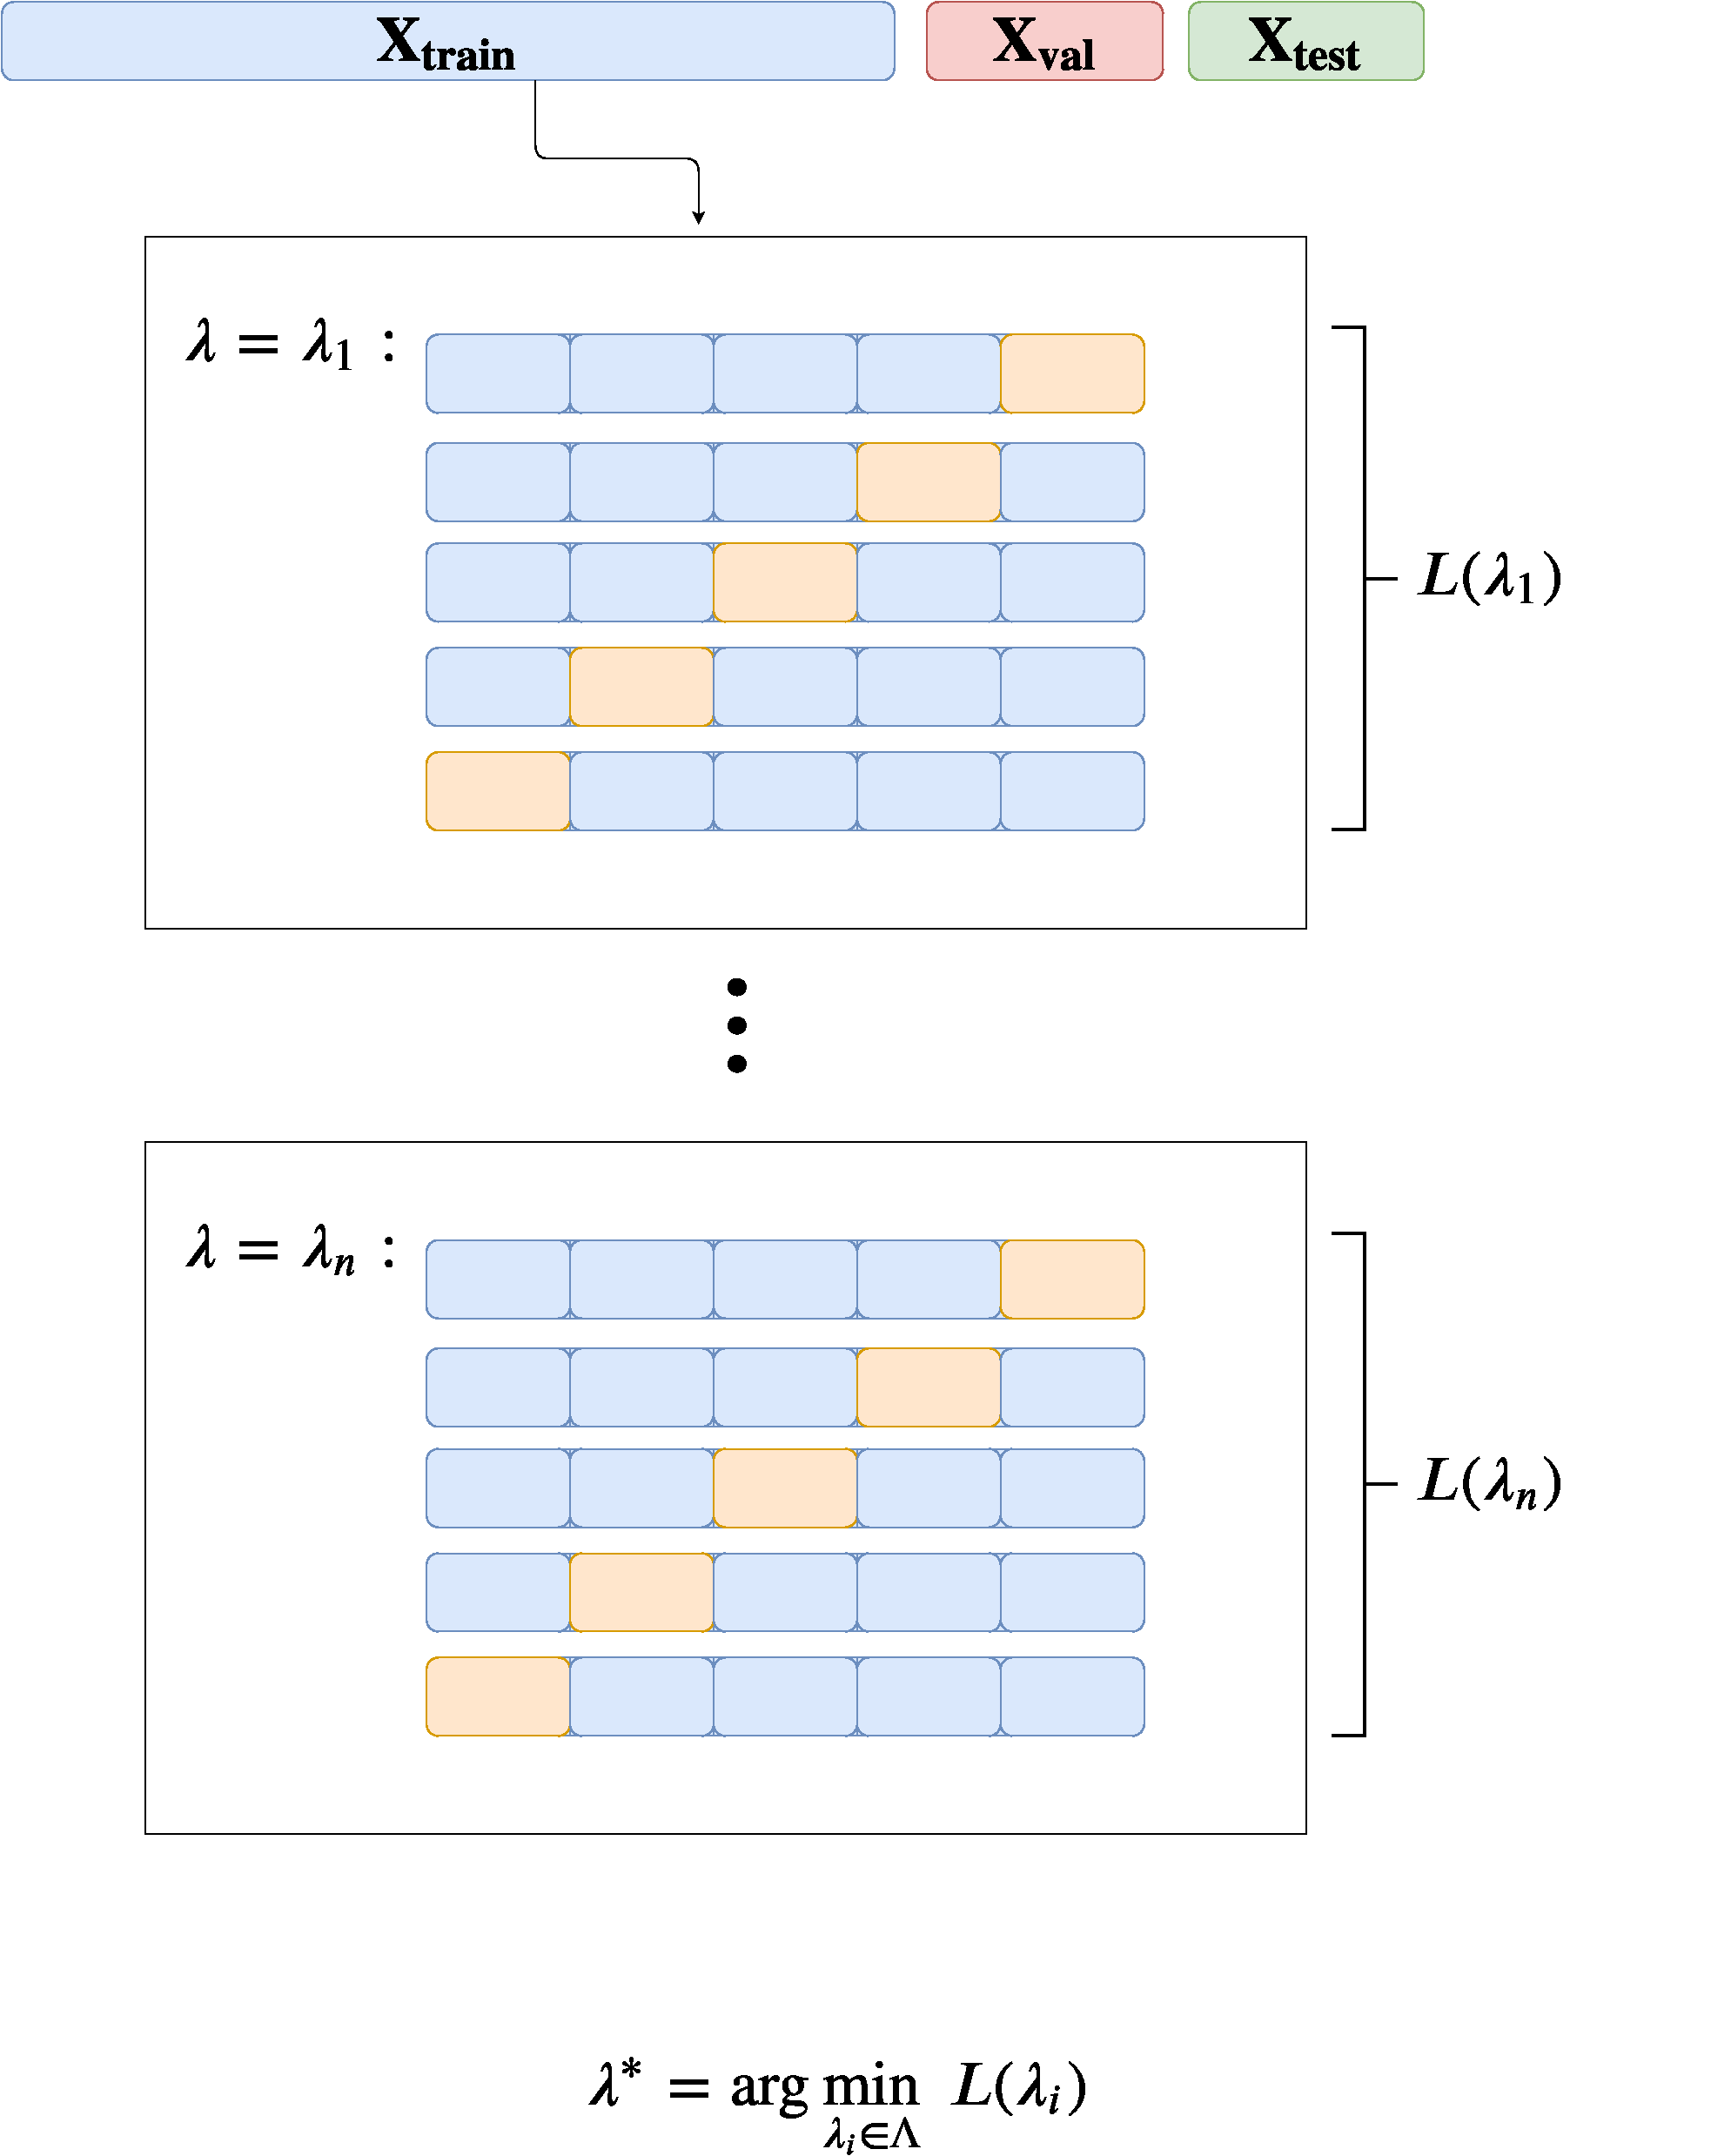
\includegraphics[width = \columnwidth]{figs/cross_val(1)(1).pdf}
    \caption{Hyperparameter selection loop for model evaluation: $\mathbf{X_{train}}$ is partitioned (here into 5). The final $\lambda^*$ is selected as the best performing $\lambda_i$ on the mean inner cross validation score, $L(\lambda_i)$. $\lambda^*$ is then used for training on $\mathbf{X_{train}}$, and this is repeated for each training split in the outer cross validation loop. }
    \label{fig:cross_val}
\end{figure*}


\subsubsection{Aitchinson Data}
The first data source that we test on is the supplementary data presented by Aitchinson [ref.]. This data is commonly used in CoDA research, and consists of 40 small sample (up to 92) compositional datasets. As part of this project, this data was digitised and uploaded to Zenodo. Zenodo is an open access research repository, and so this will allow other researchers to easily access this data in the future. The digitised data can be found here..  


\subsubsection{Metagenome data}
The next source was from a recent paper in Nature \citep{Stewart2019}, which provided the metagenome analyses from several hundred cattle rumen. The depth of each genome (this acts as a proxy for species count) is given for each of the cattle in the sample. The collection of depths per cattle is compositional, due to the capacity of the sequencing device being limited, as we saw from \cite{Gloor2017}. There were 4941 genomes identified between the 283 cattle. This data provides a good opportunity for testing the model on high dimensional data, since $d >> n$ for dimension $d$ and sample size $n$.  

\subsection{Model Tuning}
\subsubsection{Early Stopping}
Add figures and cross val results showing dip in training loss, increase in val loss and decrease in cross val performance











%%% Local Variables: 
%%% mode: latex
%%% TeX-master: "paper"
%%% End: 
